\makeatletter
\let\savedchap\@makechapterhead
\def\@makechapterhead{\vspace*{-2.4cm}\savedchap}
\chapter{Implementation}
\let\@makechapterhead\savedchap
\makeatother
\vspace*{-1.5em}
\label{chap:Implementation}
% 8 pages
After designing the overall system, the next step is to program and implement the system.
This chapter introduces three system modules, the data collection app is developed with React in section \ref{sec:Data collection web app}; the deep learning model is programmed in Python 3 with TensorFlow 2.5; adapting the model to the mobile app on Android with TensorFlow Lite and React Native framework in section \ref{sec:Mobile app implementation}.
The selection rationales of these frameworks and libraries are detailed in \ref{chap:Framework details}.

\section{Data collection web app}
\label{sec:Data collection web app}
This section introduces several key user logics and algorithms in the data collection web application.
From the user's perspective, the data collection system mainly provides three user processes: new participant registration, participant login and the core function of participant recording and uploading, which are illustrated in Figure \ref{fig:4-webapp-user-register}, \ref{fig:4-webapp-user-login} and \ref{fig:4-webapp-user-record} respectively.

Figure \ref{fig:4-webapp-user-register} shows the registration process for new participants.
According to the research ethics, each participant needs to clearly understand the research content and provide consent before registering an account.
Another worth mentioning is that the system will generate a random password in the registration process and send it to the email provided by the registrant.
This registration process can prevent the system from collecting users' private passwords.

After the registration process, Figure \ref{fig:4-webapp-user-login} depicts the authentication process for registered participant.
The participant will input the email address and the random password received during the registration process.
If a participant forgot or lost the random password, he or she can request a new random password and restart the login process.

Figure \ref{fig:4-webapp-user-record} shows the main workflow of the data collection app after the participant logs in.
In the task selection stage, the web front-end first queries the currently available tasks from the back-end and display them in a list that participant can select.
Each task has detailed text and picture descriptions, which is easy for participants to understand.

After the participant selects desired tasks, the next step is video recording.
The system uses the web real-time communication (WebRTC\footnote{Real-time communication for the web: \url{https://webrtc.org/}}) API provided in most modern browsers to record videos for the participant.
Finally, in the upload step, participants can review each recorded videos and decide whether to upload or try rerecording.

The user registration and login process in the web app adopts a common secure authentication paradigm for online applications.
Algorithm \ref{algo:User authentication} displays the process of user authentication, where the password is double hashed and salted in back-end database storage.
In addition, the system uses short-term-valid JSON Web Tokens (JWT) as the access credentials for RPC calls, also incorporating the mechanism of a periodic token refresh, which further enhances system security and protects users' privacy.

\begin{minipage}{.5\textwidth}
\begin{algorithm}[H]
\caption{User authentication}
\label{algo:User authentication}
\KwData{Email $e$, Password $p$}
\KwResult{Auth $T_a$, Refresh $T_r$}
Web browser front-end:
$EP \gets concat(e, p)$
$h \gets sha256(EP)$
$send(e, h)$\;
\BlankLine
\BlankLine
\BlankLine
\BlankLine
Back-end:
$receive(e, h)$\;
\If{user $e$ does not exist}{
    return error\;
}
\If{bcrypt hash compare $h$ failed}{
    return error\;
}
\tcp{Authenticated}
$T_a \gets JWT(\{userDetail, authUUID\})$\;
$T_r \gets JWT(refreshUUID)$\;
return $T_a, T_r$\;
\end{algorithm}
\end{minipage}
\vline
\begin{minipage}{.5\textwidth}
\begin{algorithm}[H]
\caption{Video uploading}
\label{algo:Video uploading}
\KwData{Blob video data $v$}
\KwResult{Data in chunks $c[x]$}
$s \gets 3 \times 10^{4}$ \tcp*{gRPC 32768 bytes read limit}
\For{$i \gets 0$ \KwTo $\ceil*{\frac{sizeof(v)}{s}}$}{
    $b_{left} \gets i \times s$\;
    $b_{right} \gets \max ((i+1) \times s, sizeof(v))$\;
    $c[i] \gets v[b_{left}:b_{right}]$\;
    $send(i, c[i])$\;
    $progress \gets receive()$\;
    \If{receive progress failed}{
        return error\;
    }
    $updateUI(progress)$\;
    $i \gets i+1$\;
}
\end{algorithm}
\end{minipage}

Algorithm \ref{algo:Video uploading} shows the process for segmenting large video data before uploading it to the backend server.
This segmentation algorithm runs on the browser front end, using \textit{slice} in binary large object (Blob) API for slicing the video.
The communication between the front-end and back-end uses the gRPC bidirectional streaming.
When the front-end uploads data, it also receive acknowledgement and receiving progress from the server.
 % 2 pages

\section{Mobile app implementation}
\label{sec:Mobile app implementation}
After the data collection app is implemented, the data collection process begins.
While waiting for the data set to be collected, I designed the deep model as detailed in section \ref{sec:Deep model design}.
After the design of the model is completed, the data loader and the deep model are implemented using Python programming language and TensorFlow framework.
The implementation of EfficientNet (\textit{tf.keras.applications.efficientnet.EfficientNetB0}) and the MLP classification head (\textit{tf.keras.layers.Dense} and \textit{tf.keras.layers.Dropout}) is composed directly from the TensorFlow Keras-style high-level APIs.
The Longformer implementation uses the Hugging Face Transformer\footnote{Hugging Face Transformers: \url{https://huggingface.co/transformers/}} library.
The detail of each layer in the implemented model is shown in \ref{chap:Model design details}.
After finish implementing and training the deep model, the remaining research goal is to port the deep model to Android platform.

Although the most widely used programming language for Android development is Java, this project does not use Java except for the automatically generated initialisation codes and native function bindings.
As discussed in section \ref{sec:Framework selection}, the implementation uses React Native to develop UI and application logic.
Even though JavaScript development is more convenient, it is single-threaded and is not suitable for high performance parts in the application.
For the parts that require high performance, such as the image pipeline, the anonymisation process, and the deep model inference process, the C++ programming language is used for multi-threaded Android native development.

\subsection{Architecture overview}
The architecture of the mobile application developed in this research is shown in Figure \ref{fig:4-mobile-arch}.
The arrows in the figure indicate the direction of data flow and clearly show dependencies across different functional blocks.
The left half of the figure describes the user interface and user interaction logic developed using React Native, and the right half describes the core functions of the application developed using C++.
These two parts use React Native Javascript Interface (JSI) for communication.

\begin{figure}[!ht]
    \centering
    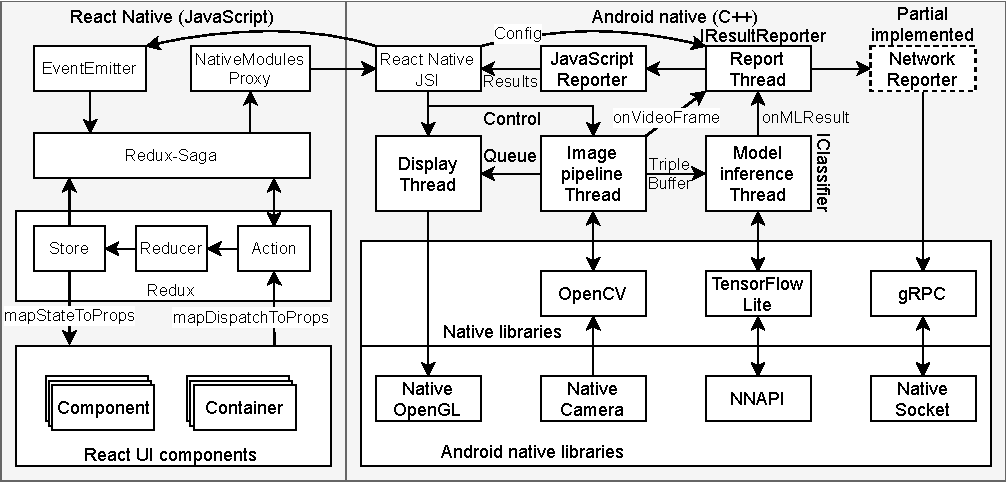
\includegraphics[width=\textwidth]{implementation/imgs/4-mobile-arch.pdf}
    \caption{Mobile app architecture and data flow}
    \label{fig:4-mobile-arch}
\end{figure}

The core functions of this project in the native part shown on the right side in Figure \ref{fig:4-mobile-arch} is much worth discussing than UI implementation on the left side.
These core functions include displaying images without lag and running model inference at the same time.
To achieve the goal, this project implements these functions in C++ by using multi-threading to enable asynchronous processing for display (a real-time task), model inference and network transmission (time-consuming tasks).
It can better take advantage of the multi-core of the mobile phone processor, and time-consuming tasks will not affect the real-time task, which ensures a smooth user experience.

\begin{figure}[!ht]
    \centering
    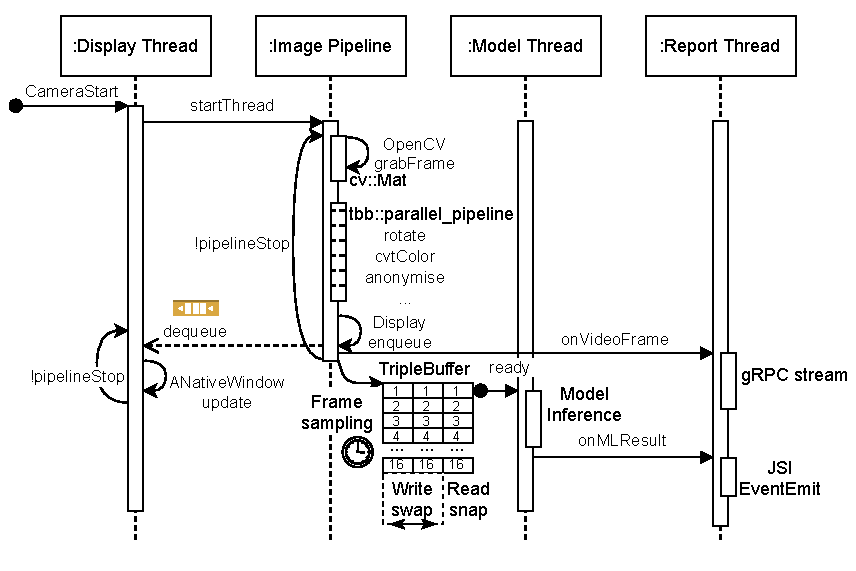
\includegraphics[width=\textwidth]{implementation/imgs/4-model-infer.pdf}
    \caption{Sequence diagram of the multi-threaded app}
    \label{fig:4-model-infer}
\end{figure}
The sequence diagram in Figure \ref{fig:4-model-infer} describes the interactions between four threads in the Android application.
After the user enters the exam screen, the display thread will receive the processed image data through a queue and update the display.
After the exam begins, the model inference thread will be started to receive processed image data from a triple buffer, and performs model inference, then informs the result report thread after getting the result.

The rest of this section will introduce in detail the multi-threaded design for the core function, including display thread, image processing pipeline thread, and model inference thread.

\subsection{Display and image processing pipeline}
This subsection introduces a real-time task involving the display and image processing pipeline in the app.
The image processing pipeline firstly receives an image from a camera on the mobile phone then transforms and anonymises it with OpenCV.
The display thread is responsible for receiving the image processed by the image processing pipeline and showing it through OpenGL.
This process is a real-time task, where the display process takes less time than the image processing process.
The display thread needs to wait for the processed image data from the processing pipeline thread.
Therefore, transferring data across two threads should use the producer-consumer programming paradigm with the blocking queue data structure.

A queue is a commonly used first-in-first-out (FIFO) data structure of a sequential organised collection of entities which can be modified by \textit{enqueue} (adding entities at one end) and \textit{dequeue} (removing entities from the other end).
A thread-safe blocking queue is a queue that may block in \textit{dequeue} operation or \textit{enqueue} operation.
If the blocking queue has already been empty, a \textit{dequeue} operation will block the calling thread until new data are available in the queue.
Conversely, a \textit{enqueue} operation will block the calling thread if the blocking queue has already full.

\begin{algorithm}[!ht]
\caption{Image processing pipeline thread}
\label{algo:Image processing pipeline thread}
\KwData{Readable image stream $v$ of cv::VideoCapture}
\KwResult{Processed image array $p$[] of cv::Mat}
initialisation\tcp*{OpenCV VideoCapture, CascadeClassifier, FacemarkLBF}
$STOP \gets false$\;
\While{not STOP}{
    $p_{bgr} \gets read(v)$\;
    $p_{grey} \gets cvtColor(p_{bgr}, BGR2GRAY)$\tcp*{Grey is used for detecting face}
    $p_{half} \gets resize(p_{grey}, 0.5f, 0.5f)$\tcp*{Scale down for better preformance}
    $p_{half} \gets equalizeHist(p_{half})$\tcp*{Histogram equalisation for better adaptation to different environmental lighting}
    $f$[] $\gets CascadeClassifier::detectMultiScale(p_{half}, parameters)$\;
    $l$[][] $\gets FacemarkLBF::fit(p_{half}, f$[]$)$\;
    \For{$i \gets 0$ \KwTo $sizeof\ f$[]}{
    $p_{anonymous} \gets drawCover(p_{bgr}, f$[$i$]$)$\;
    $p_{anonymous} \gets drawLandmark(p_{anonymous}, l$[$i$][]$)$\;
    }
    $p_{rgba} \gets cvtColor(p_{anonymous}, BGR2RGBA)$\tcp*{ANativeWindow requires image in RGBA format}
    $enqueue(displayQueue, p_{rgba})$\tcp*{Enqueue to display thread}
    $addImage(p_{anonymous})$\tcp*{Preform temporal sampling and add to the current writing queue in the triple buffer}
}
\end{algorithm}

Algorithm \ref{algo:Image processing pipeline thread} shows the simplified processing procedure in the image processing pipeline thread, which includes reading camera data, performing anonymisation, and sending the processed data to other threads.
For the display thread, it only needs to dequeue the RGBA data processed and converted by Algorithm \ref{algo:Image processing pipeline thread} from the $displayQueue$, and invoke the Android API to set the OpenGL texture.
In this way, the new frame will be displayed in real-time from the OpenGL rendering loop.

\subsection{Tensorflow Lite adoption and model inference}
Although Google provides some ready-made models and easy-to-call Java bindings, it is necessary to use C++ for custom model workflow.
Besides, not all deep models implemented in TensorFlow can be converted to the Lite version due to limited operators compatibility.
In the deep model conversion stage, this project firstly loads the trained model, then uses the \textit{from\_keras\_model} mode\footnote{TensorFlow Lite converter: \url{https://www.tensorflow.org/lite/convert\#convert_a_keras_model_}} of the TensorFlow Lite converter by specifying \textit{SELECT\_TF\_OPS}\footnote{Select TensorFlow operators: \url{https://www.tensorflow.org/lite/guide/ops_select}} parameter to allow the usage of certain TensorFlow operators in the TensorFlow Lite version.

To reduce the app size and make the converted model generated in the previous step better adapt to mobile devices, this project strips unnecessary operators by compiling the executable binary files from TensorFlow Lite source code according to the document\footnote{Reduce TensorFlow Lite binary size: \url{https://www.tensorflow.org/lite/guide/reduce_binary_size}}.
Besides, another important reason why this project chooses to compile libraries from source code is to use TFLite C++ API as documented in the official guide\footnote{Use TFLite C++ API: \url{https://www.tensorflow.org/lite/guide/android\#use_tflite_c_api}}.

One failed attempt is trying to use the built-in optimisation of the TensorFlow Lite converter, such as pruning and quantisation introduced in mobile device optimisation section \ref{sec:Mobile device optimisation}.
However, due to an unresolved issue\footnote{Did not get operators or tensors in subgraph: \url{https://github.com/tensorflow/tensorflow/issues/45313}} in the TensorFlow v2.5.0 library, further optimisation attempts are failed.
After this issue of library is solved in the future, the model should be able to be further optimised.

After converting the model into the TFLite version and building the runtime binary, then it is time to implement the model inference thread.
As mentioned earlier, the key task in the model inference thread is to use the frames received from the image processing pipeline for temporal sampling to write sampled frames to the triple buffer and invoke the TensorFlow Lite library.
The temporal sampling algorithm as shown in Algorithm \ref{algo:Temporal sampling and triple buffering} is to sample 16 images from the video stream at an equal time interval same as one iteration in the model training process (25fps).

\begin{algorithm}[!ht]
\caption{Temporal sampling and triple buffering}
\label{algo:Temporal sampling and triple buffering}
\KwData{Processed images from pipeline $x$[]; Current frame index$C_{frame}$}
\KwResult{Temporal sampled images queue $s$[$16$]; Image index array $p$[$16$]}
$T_{now} \gets getTime()$\tcp*{Assume time in second for simplex}
$T_{diff} \gets T_{now} - T_{last}$\;
$f \gets \floor*{\frac{T_{diff} \times TARGET_FPS}{10}}$\tcp*{Sampling frames at 0s(frame 0), 0.4s, 0.8s, 1.2s, 1.6s...6s(frame 15)}
\If{$f \geq MAX\_POSITION\_EMBEDDINGS - 2$}{
    \tcp{Position embedding overflown, restart frame sampling}
    $T_{last} \gets T_{now}$\;
    $C_{frame} \gets 0$\;
    empty $s$ and $p$\;
}
\If{$f \geq sizeof\ s$}{
    \tcp{Sampling a frame to the queue}
    $push(s, x)$\;
    $push(p, C_{frame})$\;
    \If{sizeof\ s == BATCH\_FRAME\_NUM}{
        \tcp{Finish sampling 16 frames}
        $T_{last} \gets T_{now}$\;
        $C_{frame} \gets 0$\;
        $flipWriter()$\tcp*{flip the triple buffer}
        empty $s$ and $p$\tcp*{clear old data after flipped to new buffer}
    }
}
\end{algorithm}

As for triple buffering, it is a bridge that connects the image processing thread and model inference thread.
This data structure type has been widely used in the producer-consumer paradigm to deal with the inconsistency of the consumer has a slower speed than the producer.
When the producer is much faster than the consumer, some data loss is inevitable, so it is only necessary to ensure that the consumer gets the latest data in this scenario.

The implementation of triple buffering is an strengthened special case of ring buffering.
In the triple buffering, there are three buffers in the memory, one is snap for reading from the consumer, and the other two are for flip writing from the producer.
When the consumer reads, the newly written buffer will become a reading snap, and then the producer will write the released buffer and the remaining buffer.
Thanks to the atomic operation support provided by C++, \citet{andre2021triple} proposed a lock-free triple buffer implementation for the processes of creating snap and flip writing.

One problem with the initial version of this project is that the model inference thread may read empty data from the triple buffer because the image processing pipeline takes time to produce.
To tinkle this problem, a \textit{readLastBlock} is implemented using mutex and a conditional variable to block the model inference thread until the first set of image data is valid.
After completing the implementation of temporal sampling and triple buffering,  this project only need to copy the reading snap into tensor and invoke the TensorFlow Lite inference API to get the result.
 % 2.5 pages
